\chapter{Full Channel, Narrowband Analysis}
\label{chap:full_narrow}

The analysis now expands from the LOS model to a more comprehensive full-channel model. This section considers the impact of Multipath components generated by reflections off the buildings lining. The analysis remains within the narrowband regime, where the channel's response can be characterized by a single complex coefficient, but this coefficient now incorporates the vector sum of all significant propagation paths, not just the direct one.


In a realistic urban environment, the signal transmitted from TX to RX does not travel along a single path. Instead, it propagates along multiple paths due to reflections from surrounding objects, in this case, the building facades. Each of these paths is an MPC. The total received signal is the vector sum of all these MPCs. The narrowband channel transfer function, previously represented by a single complex gain $\alpha_1$ for the LOS path, is now the sum of the complex gains of all MPCs:
\begin{equation}
	h_{NB} = \sum_{n=1}^{N} \alpha_n
\end{equation}
where $N$ is the total number of significant MPCs, including the LOS path and all reflected paths. Each complex gain $\alpha_n$ is a function of the path's length, the reflection coefficients of the surfaces it interacts with, and the propagation delay.

The primary tool for identifying these paths and calculating their geometry is the \textbf{image method}. For each reflecting surface, an image of the transmitter is created. A straight line from this image to the receiver identifies the path of the reflected wave, as shown in Figure \ref{fig:image_method_single}. This method can be extended recursively to find paths with multiple reflections.

\begin{figure}[h!]
	\centering
	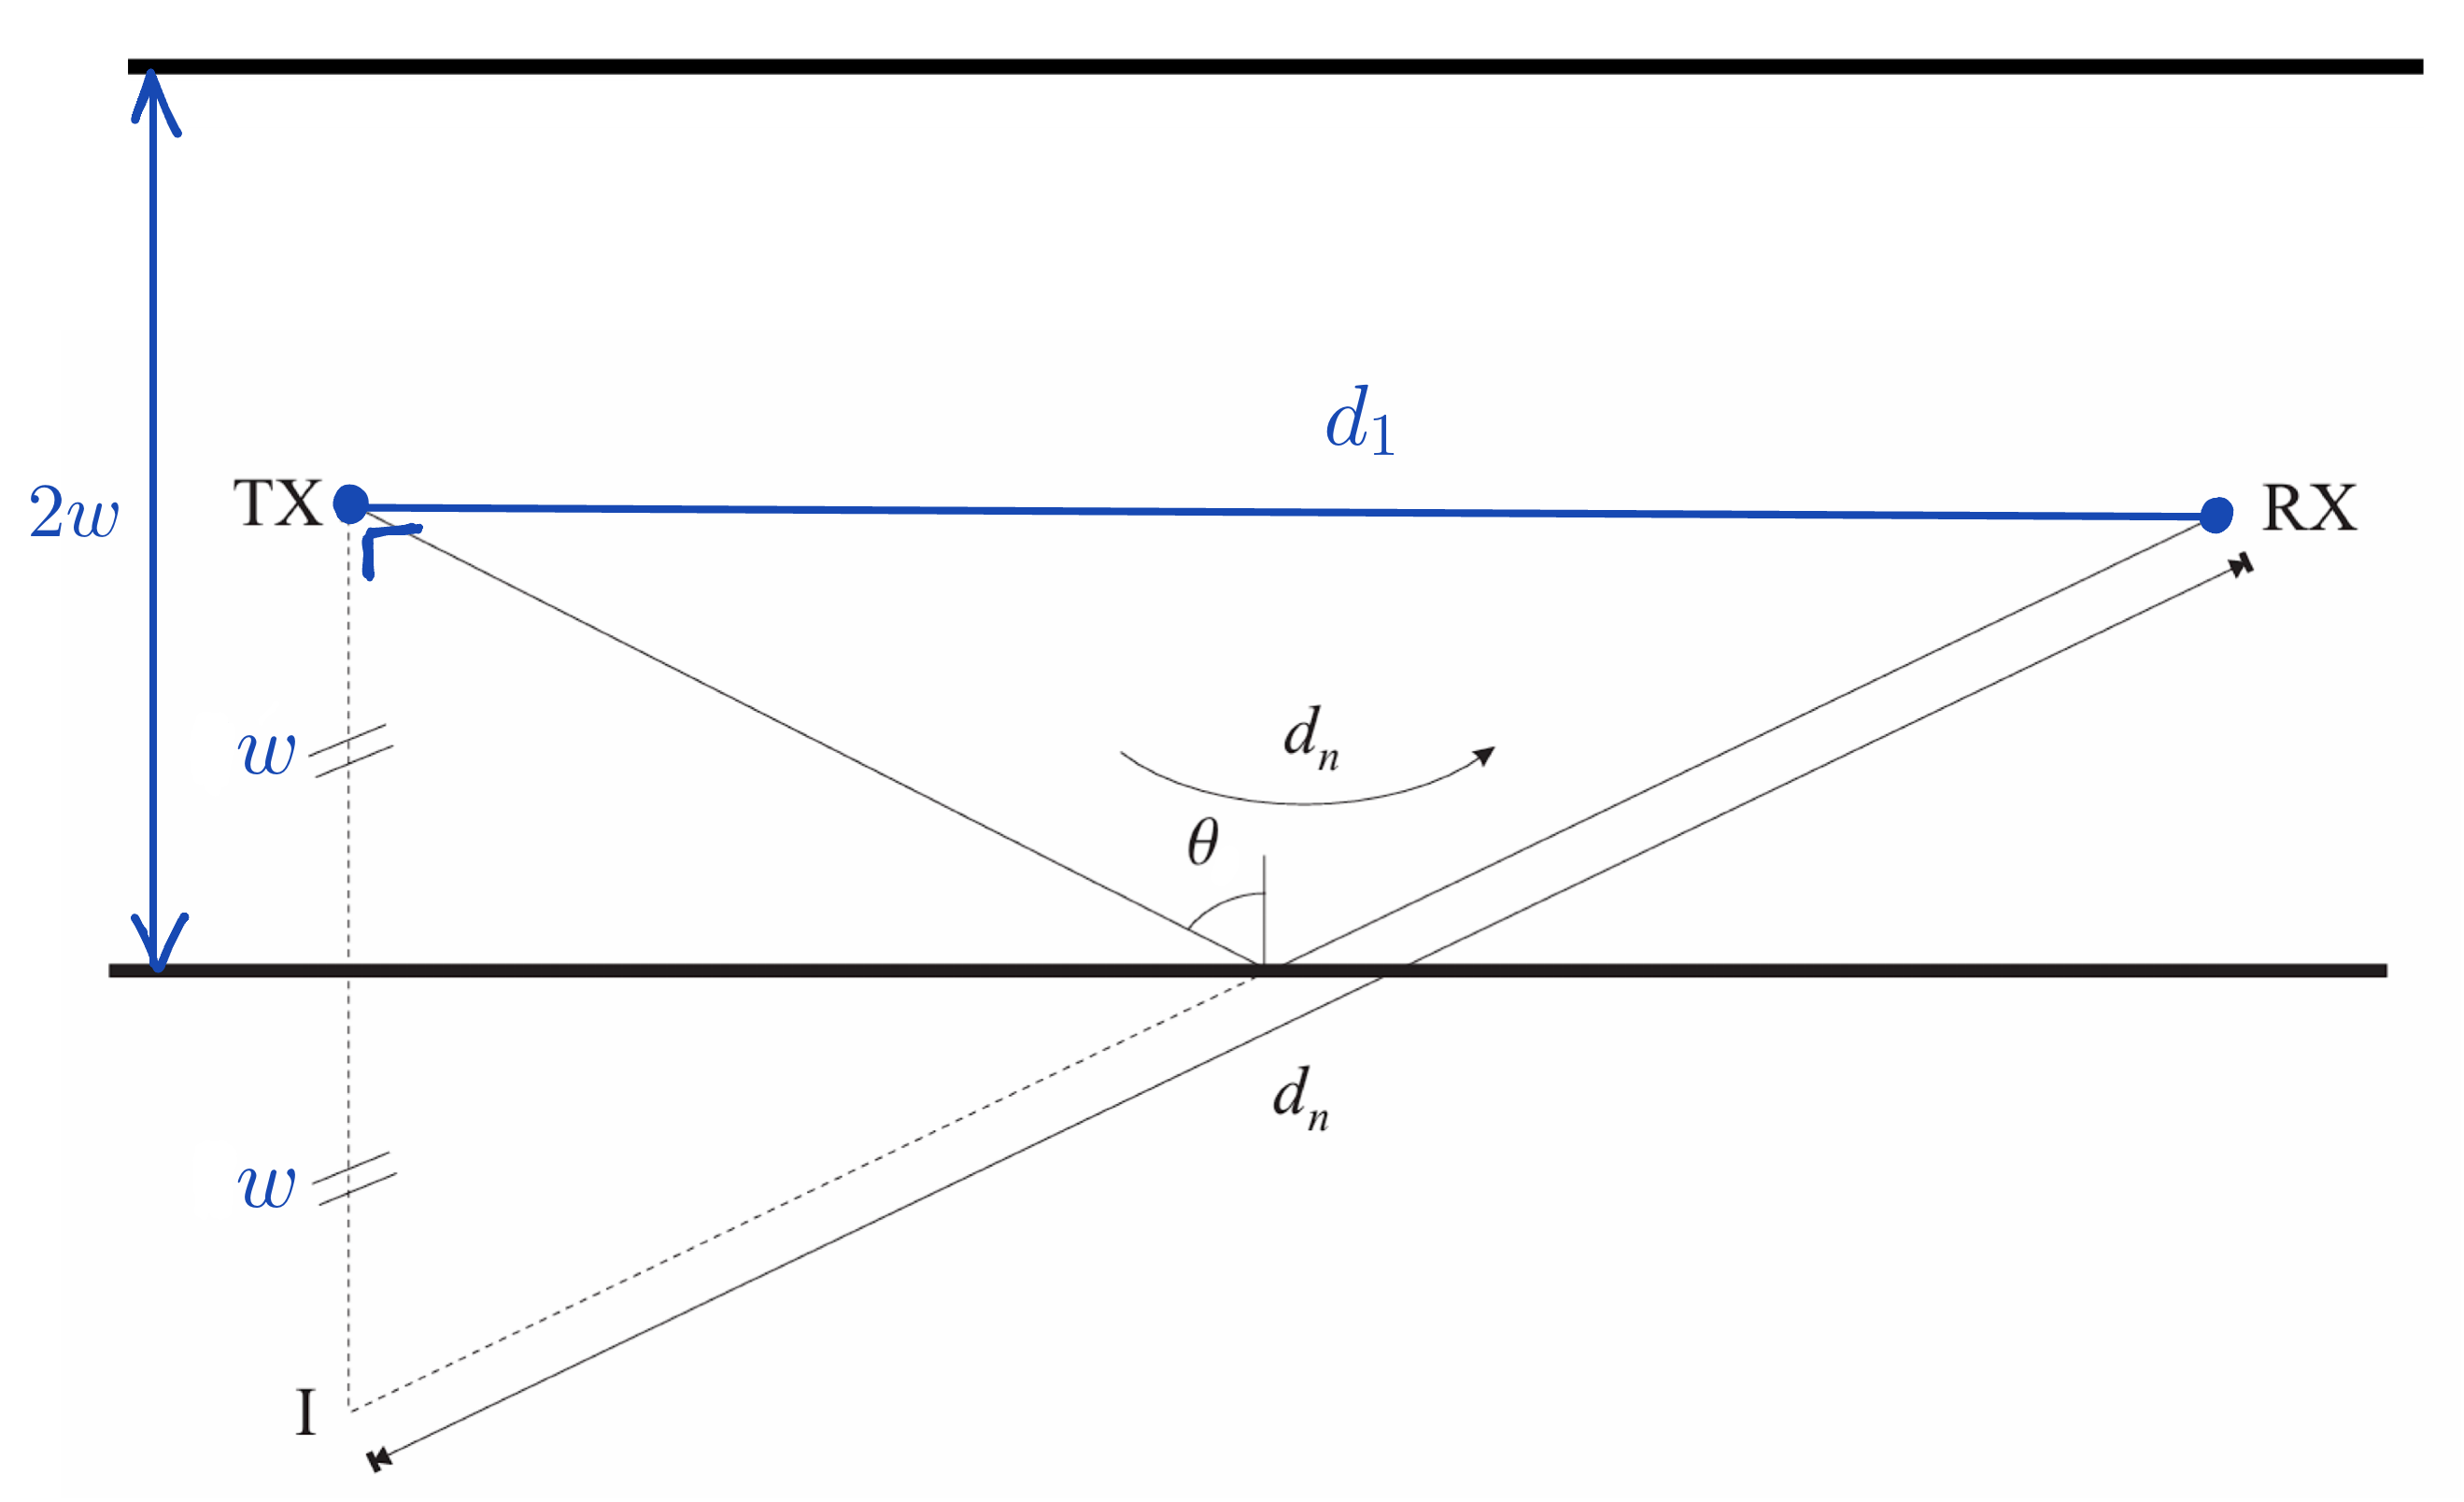
\includegraphics[width=0.7\linewidth]{content/4-images/image-method.png}
	\caption{The image method for a single reflection. The path of the reflected ray from TX to RX is found by drawing a straight line from the image transmitter I to RX.}
	\label{fig:image_method_single}
\end{figure}


\section{Multipath Component Geometry}
The scenario is an urban canyon of width $2w = 20$ m. The TX and RX are in the center of the street, separated by a distance $d_1$. The walls of the canyon are at $y = w$ and $y = -w$. We consider up to triple reflections.

\subsubsection{Line-of-Sight (LOS) Path}
This is the direct path between TX and RX, denoted as path $n=1$.
\begin{itemize}
	\item \textbf{Path Length:} $d_1$
	\item \textbf{Propagation Delay:}
	\begin{equation}
		\tau_1 = \frac{d_1}{c}
	\end{equation}
\end{itemize}

\subsubsection{Single Reflection Paths}
There are two paths involving a single reflection, one off each building wall.
\begin{itemize}
	\item \textbf{Path Length ($d_2$):} Using the image method, the path length is the hypotenuse of a right triangle with legs $d_1$ and $2w$.
	\begin{equation}
		d_2 = \sqrt{d_1^2 + (2w)^2}
	\end{equation}
	\item \textbf{Propagation Delay ($\tau_{2}$):}
	\begin{equation}
		\tau_{2} = \frac{\sqrt{d_1^2 + (2w)^2}}{c}
	\end{equation}
	\item \textbf{Angle of Incidence ($\theta_{i,2}$):} The angle of incidence and reflection is:
	\begin{equation}
		\cos(\theta_{i,2}) = \frac{d_1}{d_2} = \frac{d_1}{\sqrt{d_1^2 + (2w)^2}}
	\end{equation}
\end{itemize}

\subsubsection{Double Reflection Paths}
There are two paths involving two reflections (e.g., Wall 1 $\rightarrow$ Wall 2 $\rightarrow$ RX).
\begin{itemize}
	\item \textbf{Path Length ($d_3$):}
	\begin{equation}
		d_3 = \sqrt{d_1^2 + (4w)^2}
	\end{equation}
	\item \textbf{Propagation Delay ($\tau_{3}$):}
	\begin{equation}
		\tau_{3} = \frac{\sqrt{d_1^2 + (4w)^2}}{c}
	\end{equation}
\end{itemize}

\subsubsection{Triple Reflection Paths}
There are two paths involving three reflections.
\begin{itemize}
	\item \textbf{Path Length ($d_4$):}
	\begin{equation}
		d_4 = \sqrt{d_1^2 + (6w)^2}
	\end{equation}
	\item \textbf{Propagation Delay ($\tau_{4}$):}
	\begin{equation}
		\tau_{4} = \frac{\sqrt{d_1^2 + (6w)^2}}{c}
	\end{equation}
\end{itemize}
The total number of MPCs for up to 3 reflections is $N=1+2+2+2=7$ paths.

\begin{figure}[H]
	\centering
	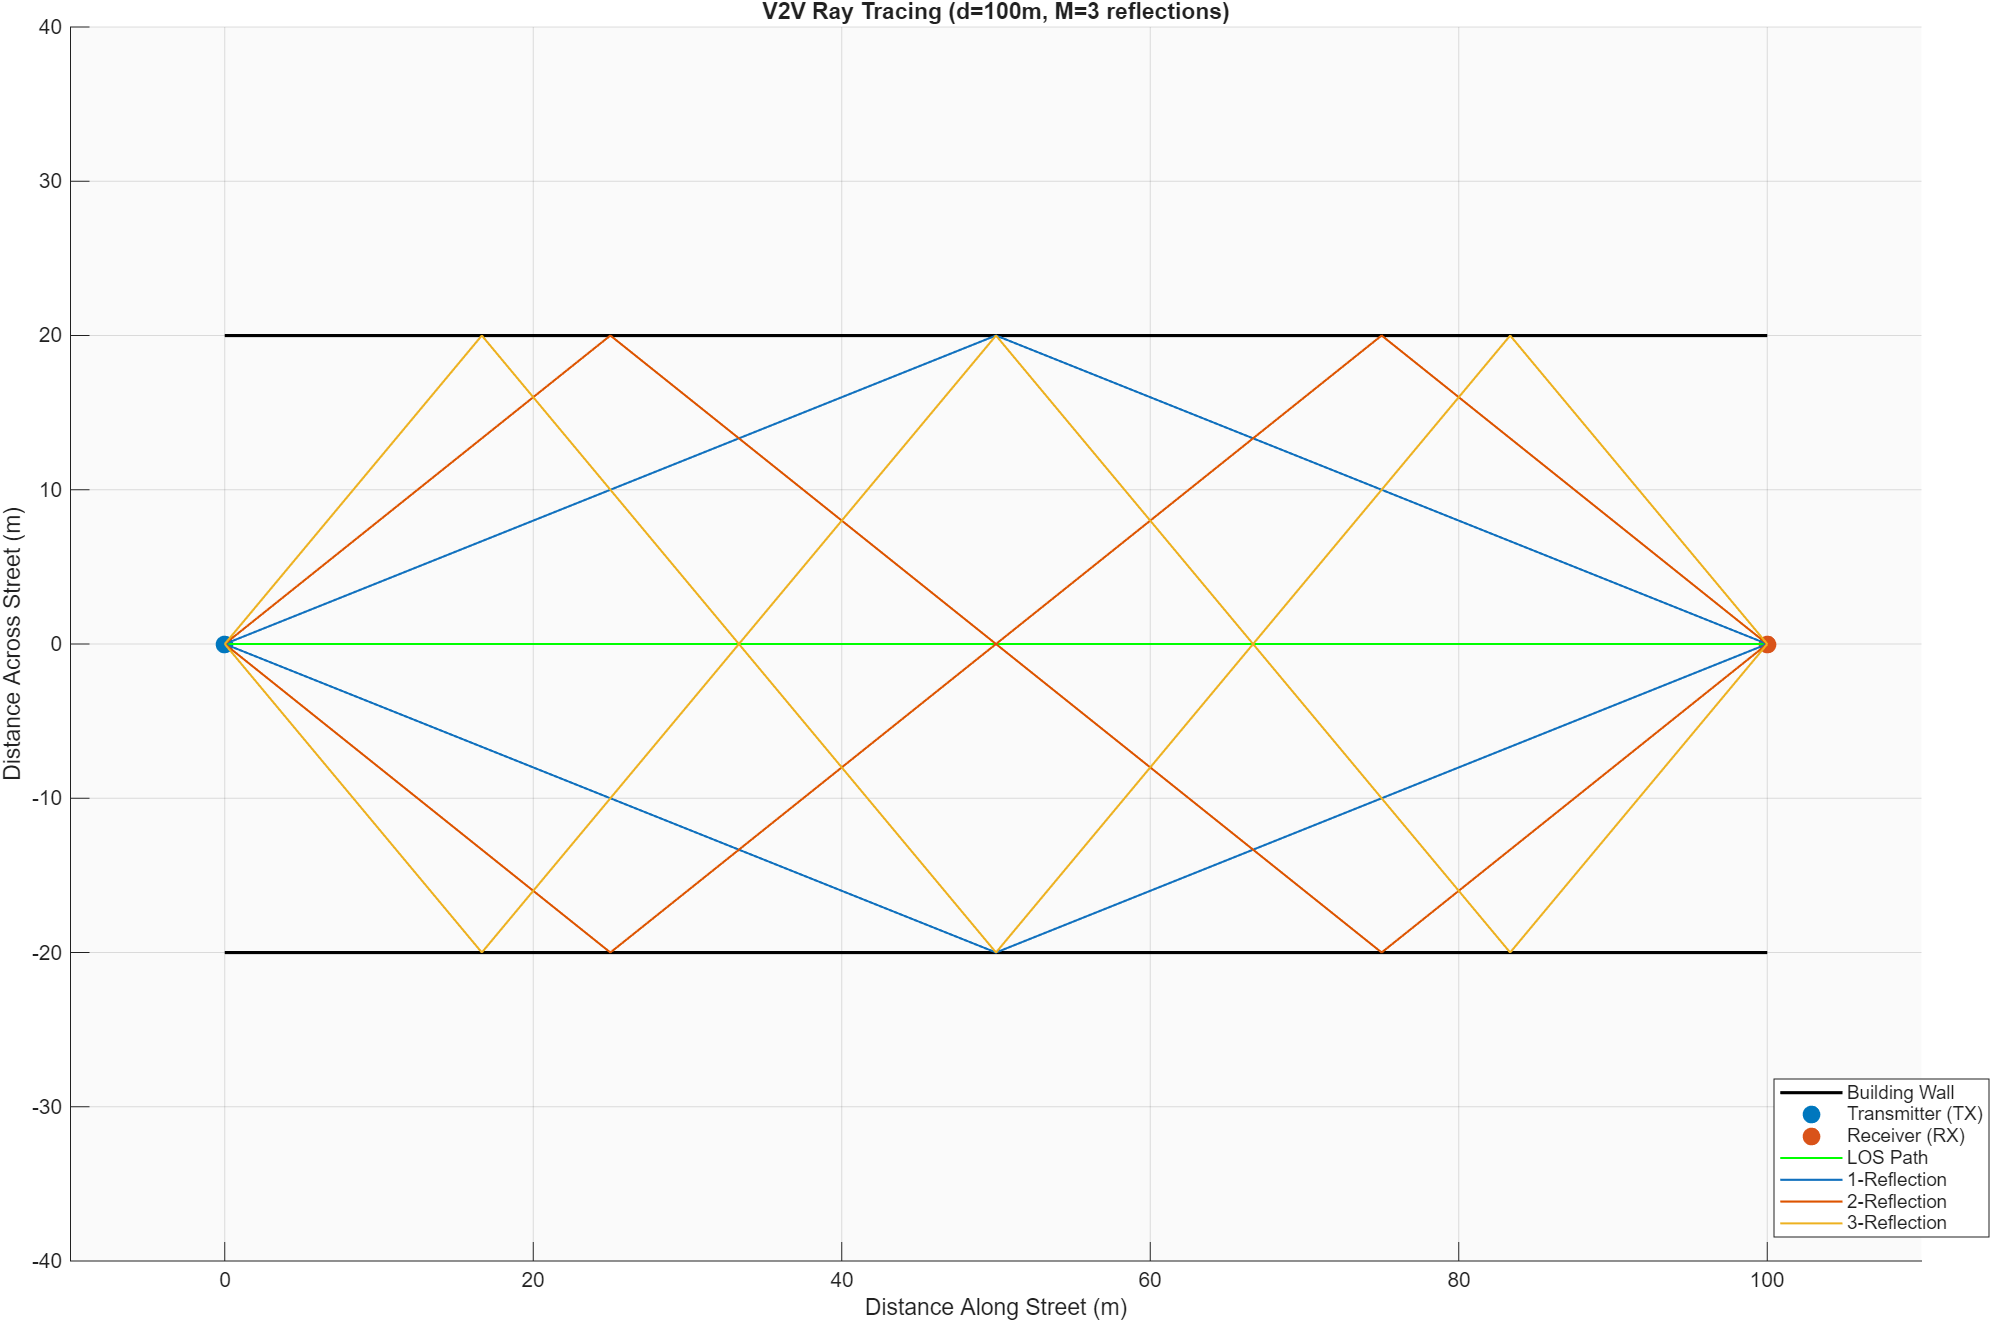
\includegraphics[width=\linewidth]{content/4-images/ray-tracing-3-reflect}
	\caption{Simulation of the Image method ray-tracing for 3 reflections}
	\label{fig:raytracing-3reflex}
\end{figure}


\section{Total Received Voltage}
The complex amplitude $\alpha_n$ for each path $n$ must account for the path loss and any phase changes from reflections. The general form for the complex amplitude of a path of length $d_n$ with $k$ reflections is:
\begin{equation}
	\alpha_n = \left( j \frac{\lambda Z_0}{4\pi^2 R_a d_n} e^{-j2\pi f_c \tau_n} \right) \times (\Gamma_{\perp}(\theta_{i,n}))^k
\end{equation}
where $\Gamma_{\perp}$ is the reflection coefficient for perpendicular polarization for the $n$-th MPC experiencing $k$ reflections:
\begin{equation}
	\Gamma_{\perp}(\theta_i) = \frac{\cos\theta_i - \sqrt{\epsilon_r - \sin^2\theta_i}}{\cos\theta_i + \sqrt{\epsilon_r - \sin^2\theta_i}}
\end{equation}
with $\epsilon_r = 4$ for the buildings. The angle of incidence $\theta_i$ is specific to each reflection order.

The total narrowband channel gain is the sum of the complex amplitudes of all 7 MPCs:
\begin{equation}
	h_{NB} = \alpha_{LOS} + \sum_{n \in SR} \alpha_n + \sum_{n \in DR} \alpha_n + \sum_{n \in TR} \alpha_n
\end{equation}
where SR, DR, and TR denote the sets of single, double, and triple reflection paths. The total received voltage $\underline{V}_{RX}$ is then:
\begin{equation}
	\underline{V}_{RX} = \frac{h_{NB}}{2} \underline{V}_{TX}
\end{equation}

\section{Received Power and Comparison with Friis Formula}
The narrowband transfer function found in in Equation \eqref{eq:narrow} is given by :
\begin{equation}
	h_{NB} = \sum_{n=1}^{N=7} \alpha_n
\end{equation}
The received power is therefore:
\begin{equation}
	P_{RX} = |h_{NB}|^2 P_{TX} = \left| \sum_{n=1}^{N=7} \alpha_n \right|^2 P_{TX}
\end{equation}
This expression highlights the difference from the LOS-only case. The Friis formula, derived in Chapter \ref{chap:los}, predicts the received power based on a single, unobstructed path:
\begin{equation}
	P_{RX, \text{Friis}} = P_{TX} G_{TX} G_{RX} \left( \frac{\lambda}{4\pi d} \right)^2 = |\alpha_{LOS}|^2 P_{TX}
\end{equation}
The Friis formula represents the power of only the first term ($n=1$) in the sum. In the full channel model, the total power depends on the vector sum of all 7 MPCs. Because the paths have different lengths $d_n$ and undergo different phase shifts ($e^{-j2\pi f_c \tau_n}$ and from reflections), the complex amplitudes $\alpha_n$ add up coherently.

This coherent summation results in multipath fading. Unlike the monotonic decrease of power with distance predicted by the Friis formula, the full-channel received power will exhibit significant fluctuations as the distance $d$ changes.
\begin{itemize}
	\item \textbf{Constructive Interference:} At locations where the MPCs arrive largely in-phase, their amplitudes add up, resulting in a received power that can be significantly higher than the Friis prediction.
	\item \textbf{Destructive Interference:} At locations where some MPCs arrive out-of-phase, their amplitudes cancel each other out, leading to deep nulls or "fades" in the received power, where it can drop far below the Friis prediction.
\end{itemize}
Figure \ref{fig:prx_vs_friis} illustrates this comparison. The plot shows the calculated instantaneous received power $P_{RX}$ as a function of distance, overlaid with the smooth decay curve of the Friis formula. The rapid oscillations of the actual power around the Friis curve are the hallmark of a multipath environment.

\begin{figure}[h!]
	\centering
	% You should generate this plot using simulation tools (e.g., MATLAB, Python)
	% based on the derived equations for the 7 MPCs.
	\includegraphics[width=0.9\linewidth]{content/4-images/prx_vs_friis_placeholder.png} % Placeholder path
	\caption{Comparison of the total received power in the full multipath channel versus the power predicted by the Friis formula. The Friis formula (dashed line) represents the LOS power, while the actual power (solid line) shows significant fading due to multipath interference.}
	\label{fig:prx_vs_friis}
\end{figure}

\section{Rician K-factor}
The Rician K-factor is a key parameter that quantifies the severity of fading in a channel. It is defined as the ratio of the power in the dominant, specular component (in this case, the LOS path) to the total power in the scattered, non-line-of-sight (NLOS) components.
\begin{equation}
	K = \frac{\text{Power in LOS component}}{\text{Power in NLOS components}} = \frac{P_{LOS}}{P_{NLOS}}
\end{equation}
The power of an individual path $n$ is given by $P_n = |\alpha_n|^2 P_{TX}$. Therefore, the K-factor can be expressed in terms of the complex amplitudes $\alpha_n$:
\begin{equation}
	K = \frac{|\alpha_{LOS}|^2}{\sum_{n=2}^{7} |\alpha_n|^2}
\end{equation}
To evaluate this, we need to express $|\alpha_n|^2$ in terms of physical parameters. From the LOS analysis in Chapter \ref{chap:los}, we found that the received power for the direct path is identical to the Friis formula:
\begin{equation}
	P_{LOS} = |\alpha_{LOS}|^2 P_{TX} = G_{TX} G_{RX} \left( \frac{\lambda}{4\pi d} \right)^2 P_{TX}
\end{equation}
This gives us the power gain for the LOS component ($d_1=d$, $|\Gamma_1|^2=1$):
\begin{equation}
	|\alpha_{LOS}|^2 = G_{TX} G_{RX} \left( \frac{\lambda}{4\pi d} \right)^2
\end{equation}
For any other multipath component $n$, which experiences reflections, the power is reduced by the cumulative reflection coefficient $\Gamma_n$. The power gain for a reflected path of length $d_n$ is therefore:
\begin{equation}
	|\alpha_n|^2 = G_{TX} G_{RX} \left( \frac{\lambda}{4\pi d_n} \right)^2 |\Gamma_n|^2
\end{equation}
where $\Gamma_n$ is the product of the reflection coefficients for path $n$. Substituting these expressions for power gain into the K-factor equation:
\begin{equation}
	K = \frac{G_{TX} G_{RX} \left( \frac{\lambda}{4\pi d} \right)^2}{\sum_{n=2}^{7} G_{TX} G_{RX} \left( \frac{\lambda}{4\pi d_n} \right)^2 |\Gamma_n|^2}
\end{equation}
The common terms, including antenna gains and wavelength, cancel out, leaving a purely geometric relationship:
\begin{equation}
	K = \frac{\frac{1}{d^2}}{\sum_{n=2}^{7} \frac{|\Gamma_n|^2}{d_n^2}} = \frac{1}{d^2 \sum_{n=2}^{7} \frac{|\Gamma_n|^2}{d_n^2}}
\end{equation}
A high K-factor indicates that the channel is dominated by the LOS path, and fading will be less severe (Rician fading). A low K-factor indicates that the scattered paths are strong relative to the LOS path, leading to deep fades characteristic of Rayleigh-like fading.

\section{Path Loss Model}
To analyze the large-scale path loss, we must average out the small-scale fading caused by the rapid phase changes of the MPCs. This is done by computing the average received power, $\langle P_{RX} \rangle$, over local areas, defined as 5m segments. This averaging smooths out the fast fluctuations, revealing the slower trend of power decay with distance.
\begin{equation}
	\langle P_{RX}(d) \rangle = \frac{1}{5m} \int_{d-2.5m}^{d+2.5m} P_{RX}(x) dx
\end{equation}
We then fit a path loss model of the canonical form to these averaged values:
\begin{equation}
	L(d) [dB] = L(d_0) + 10n \log_{10}\left(\frac{d}{d_0}\right)
\end{equation}
where $L(d) = 10 \log_{10}(P_{TX} / \langle P_{RX}(d) \rangle)$, $d_0$ is a reference distance (e.g., 1m), and $n$ is the path loss exponent. This exponent describes how quickly the signal attenuates with distance on a large scale.

\section{Variability $\sigma_L$}
The variability, or shadowing standard deviation $\sigma_L$, quantifies the variation of the actual received power around the path loss model prediction. It is calculated as the standard deviation of the difference (in dB) between the local-area averaged power and the path loss model prediction.
\begin{equation}
	\sigma_L^2 = \text{Var} \left[ 10\log_{10}(\langle P_{RX} \rangle) - (P_{TX}[dBm] - L(d)[dB]) \right]
\end{equation}

\section{Fade Margin and Cell Range}
Assuming the power variations around the path loss model are log-normally distributed, we can determine the fade margin ($M$) required to achieve a certain communication reliability. The reliability is the probability that the received power is above the receiver sensitivity ($P_{sens} = -70$ dBm).
\begin{equation}
	\text{Pr}(P_{RX} > P_{sens}) = \text{Reliability}
\end{equation}
The fade margin is the extra power (in dB) needed to overcome fading. The maximum allowable path loss for a given reliability is $L_{max} = P_{TX}[dBm] - P_{sens}[dBm] - M$. The cell range is the distance $d$ at which the path loss $L(d)$ equals this maximum allowable path loss. We can calculate the required margin for 50\%, 95\%, and 99\% reliability and the corresponding cell ranges.

\section{Interpretation of Results}
The introduction of reflections from buildings fundamentally changes the channel behavior compared to the simple LOS case.
\begin{itemize}
	\item \textbf{Multipath Fading:} The total received power is no longer a monotonic function of distance. The vector sum of the MPCs creates an interference pattern, causing rapid and deep fluctuations in signal strength (fading) as the distance $d$ changes. This is a critical feature of real-world urban channels.
	\item \textbf{Rician K-factor:} The K-factor provides a quantitative measure of the channel's nature. For short distances $d$, the LOS path is much stronger than the reflected paths, resulting in a high K-factor and a Rician-like distribution with moderate fading. As $d$ increases, the LOS power decreases, and the reflected paths become relatively more significant, lowering the K-factor and making the channel behave more like a Rayleigh fading channel.
	\item \textbf{Path Loss Exponent:} The path loss exponent $n$ derived from the averaged power will likely be greater than 2 (the free-space value). This is because the multipath environment tends to confine the energy, creating a "waveguide" effect that can alter the rate of power decay with distance.
	\item \textbf{Fade Margin and Reliability:} The variability $\sigma_L$ necessitates a fade margin to ensure reliable communication. A higher desired reliability (e.g., 99\% vs. 95\%) requires a larger fade margin, which in turn reduces the maximum communication range for the system. This highlights the trade-off between reliability and coverage in a fading channel.
\end{itemize}
